% =====================================================================
% Informe técnico — Proyecto 2: brigadas móviles de atención nutricional
% Compilar en Overleaf con pdfLaTeX. Estructura según la guía oficial.
%
% PENDIENTES: \pendiente{...} genera un recuadro naranja y una entrada en la
% "Lista de pendientes" al inicio. Para la versión final, cambiar
% [colorinlistoftodos] por [disable] en el paquete todonotes y borrar
% \listoftodos.
% \pend{...} es la versión corta (texto rojo) para usar dentro de tablas.
%
% Todas las cifras provienen de resultados/ del repositorio (ejecución
% reproducible del 2026-11-08).
% =====================================================================
\documentclass[11pt,letterpaper]{article}

\usepackage[utf8]{inputenc}
\usepackage[T1]{fontenc}
\usepackage{lmodern}
\usepackage[spanish,es-tabla,es-nodecimaldot,es-noshorthands]{babel}
\usepackage[margin=2.5cm]{geometry}
\usepackage{amsmath,amssymb}
\usepackage{graphicx}
\usepackage{booktabs}
\usepackage{tabularx}
\usepackage{array}
\usepackage{enumitem}
\usepackage{xcolor}
\usepackage[colorinlistoftodos,textsize=small]{todonotes}
\usepackage[hidelinks]{hyperref}

\newcommand{\pendiente}[1]{\todo[inline,color=orange!25]{\textbf{Pendiente:} #1}}
\newcommand{\pend}[1]{\textcolor{red!70!black}{[#1]}}
\newcommand{\cod}[1]{\texttt{#1}}
\renewcommand{\listtodoname}{Lista de pendientes}
\newcolumntype{L}{>{\raggedright\arraybackslash}X}

\begin{document}

% ---------------------------------------------------------------------
% Portada
% ---------------------------------------------------------------------
\begin{titlepage}
  \centering
  {\large \pend{Universidad} \par}
  {\large \pend{Facultad / Departamento} \par}
  \vspace{1.5cm}
  {\large Modelación y Simulación — Proyecto 2 \par}
  \vspace{2cm}
  {\LARGE\bfseries Simulación y optimización de la asignación territorial\\[4pt]
   de brigadas móviles de atención nutricional en Guatemala \par}
  \vspace{0.8cm}
  {\large Caso piloto: departamento de Chiquimula \par}
  \vspace{2.5cm}
  \begin{tabular}{ll}
    Integrante 1 & \pend{nombre y carné} \\
    Integrante 2 & Denis Rodríguez \pend{confirmar nombre y carné} \\
    Integrante 3 & \pend{nombre y carné} \\
  \end{tabular}
  \vfill
  {\large \pend{Catedrático} \par}
  \vspace{0.3cm}
  {\large Guatemala, 9 de noviembre de 2026 \par}
\end{titlepage}

\listoftodos
\clearpage
\tableofcontents
\clearpage

% ---------------------------------------------------------------------
\section*{Resumen}
\addcontentsline{toc}{section}{Resumen}

Se construyó un sistema reproducible de apoyo a decisiones que compara una asignación territorial base de brigadas móviles de atención nutricional contra una asignación optimizada con un algoritmo genético con restricciones. La demanda municipal se estima con los casos registrados de desnutrición aguda en menores de cinco años publicados por el MSPAS y las proyecciones de población del INE, para el departamento piloto de Chiquimula (11 municipios).

El modelo de demanda, elegido con un protocolo fijado de antemano, ordena correctamente a los municipios por carga (Spearman $=0.938$ frente a los registros reservados de 2023--2024), pero subestima el nivel total en un 37.9\,\%.

En la condición nominal (3 brigadas de 221 casos/año y radio de 22 km), el algoritmo genético eleva la cobertura simulada de 77.7\,\% a 92.0\,\%: \textbf{+14.3 puntos porcentuales} (IC 95\,\%: 11.7 a 16.8) en 30 réplicas pareadas, a cambio de una mayor distancia media de atención. La ventaja se reduce cuando la capacidad se satura (demanda $\times1.6$: +1.8 pp) y desaparece cuando la distancia deja de limitar (radio de 40 km: +0.2 pp). Con los casos reales de 2023 y 2024, cuya demanda supera ampliamente la capacidad, la diferencia es de +0.5 y 0.0 pp. El algoritmo alcanzó el óptimo exacto en las 150 ejecuciones. En un análisis adicional a mayor escala (Huehuetenango y el país completo), supera a la búsqueda aleatoria con el mismo presupuesto en 118 de 120 casos, pero una heurística voraz lo supera a escala nacional.

Como propuesta, un estudio de tamizaje modela que las brigadas \emph{evalúan niños} (20 a 35 evaluaciones por día, según el PMA) e \emph{identifican casos} según la tasa de cada municipio, con tiempos de viaje por carretera. Para identificar el 80\,\% de los casos esperados, Chiquimula necesita entre 5 y 8 brigadas según su productividad. Con 27.5 evaluaciones por día, 6 brigadas (dos en Jocotán, dos en Camotán, una en Esquipulas y una en Quezaltepeque) identifican el 83\,\% de los casos evaluando al 71\,\% de los niños. Orientar las brigadas por tasa encuentra 8 puntos más de casos que evaluar a la misma cantidad de niños sin priorizar.

Todos los resultados de cobertura son \textbf{simulados} bajo supuestos declarados: no representan una reducción real de la desnutrición ni una recomendación operativa para el MSPAS.

% ---------------------------------------------------------------------
\section{Problema}
\label{sec:problema}

\subsection{Contexto}

El Ministerio de Salud Pública y Asistencia Social (MSPAS) publica los casos registrados de desnutrición aguda en menores de cinco años por año, departamento, municipio, grupo etario y sexo, de 2012 a 2024~\cite{mspas}. En ese periodo el archivo suma 239{,}805 casos registrados a nivel nacional, con un aumento marcado desde 2020: 15{,}547 casos en 2019 frente a 27{,}068 en 2020 y 27{,}795 en 2024.

La desnutrición en la primera infancia es un problema persistente en Guatemala: según la Encuesta Nacional de Salud Materno Infantil 2014--2015, la más reciente de alcance nacional, la desnutrición crónica afectaba al 46.5\,\% de los menores de cinco años~\cite{ensmi}. Este proyecto trabaja con la \emph{desnutrición aguda}, que es la que registra el MSPAS en los datos usados y la que buscan y tratan los equipos de campo.
\pendiente{Confirmar la cifra de 46.5\,\% en el informe final de la ENSMI (FR318); se verificó en documentos del SIINSAN, pero no en el PDF original.}

Para detectar y tratar la desnutrición aguda en las comunidades más alejadas y de difícil acceso, el MSPAS opera \textbf{brigadas de salud y nutrición}: equipos de una nutricionista, tres auxiliares de enfermería y un piloto que hacen evaluaciones nutricionales en visitas domiciliarias, entregan micronutrientes y desparasitan a menores de cinco años. UNICEF las apoyó desde 2018 con más de 72 equipos hasta que el MSPAS las institucionalizó~\cite{unicef2024}. Como el número de equipos es limitado, decidir desde dónde opera cada uno y a qué municipios atiende es un problema de asignación territorial, que es el que aborda este proyecto con una abstracción de esas brigadas.

\subsection{Problema concreto}

Con un número limitado de brigadas móviles, cada una con capacidad finita y radio de acceso limitado, ¿desde qué municipios conviene operar y a qué municipios atender para cubrir la mayor parte posible de la demanda?

\textbf{Pregunta de investigación:} ¿Cómo puede optimizarse la ubicación y asignación de un número limitado de brigadas móviles para aumentar la cobertura simulada de la demanda municipal de atención nutricional, respetando restricciones de capacidad y acceso territorial?

Una \emph{brigada} es una unidad abstracta de capacidad móvil: tiene un municipio base, municipios atendidos, capacidad por periodo y distancia máxima de servicio. No se modelan diagnóstico, tratamiento, insumos, personal individual ni pacientes identificables.

\subsection{Lo que el estudio no puede afirmar}

\begin{itemize}[nosep]
  \item Que se redujo la desnutrición real.
  \item Que la distribución propuesta deba aplicarla el MSPAS.
  \item Que los casos registrados representen toda la prevalencia.
  \item Que una distancia geodésica equivalga a un tiempo real de viaje.
\end{itemize}

% ---------------------------------------------------------------------
\section{Objetivos}
\label{sec:objetivos}

\textbf{Objetivo general.} Comparar, mediante simulación reproducible, la cobertura de demanda municipal que logra una heurística base de ubicación de brigadas frente a una ubicación optimizada con un algoritmo genético con restricciones, en el departamento de Chiquimula.

\textbf{Objetivos específicos (medibles).}
\begin{enumerate}[label=O\arabic*.]
  \item Construir un panel municipio-año reproducible que una casos registrados, población de 0--4 años y referencia geográfica. \emph{Indicador:} 100\,\% de los municipios del piloto unidos de forma auditable y fuentes verificadas por SHA-256.
  \item Estimar la demanda municipal con datos de 2015--2022 y cuantificar su error contra los registros reservados de 2023--2024. \emph{Indicadores:} MAE, WAPE, sesgo y correlación de Spearman del ranking municipal.
  \item Estimar la diferencia de cobertura simulada entre la política base y el algoritmo genético con 30 réplicas pareadas por condición. \emph{Indicadores:} diferencia media, dispersión e intervalo de confianza del 95\,\%.
  \item Cuantificar la sensibilidad de esa diferencia ante una demanda $\times1.2$ y $\times1.6$, una capacidad $-20\,\%$ y un radio de acceso de 40 km.
  \item Verificar la calidad del algoritmo genético contra el óptimo exacto. \emph{Indicador:} brecha relativa del objetivo frente a la enumeración exhaustiva.
\end{enumerate}

% ---------------------------------------------------------------------
\section{Fuentes}
\label{sec:fuentes}

\subsection{Datos utilizados}

\begin{table}[htbp]
\centering
\small
\begin{tabularx}{\textwidth}{>{\raggedright\arraybackslash}p{3.2cm}L>{\raggedright\arraybackslash}p{2.4cm}L}
\toprule
Fuente & Contenido & Licencia & Clasificación \\
\midrule
MSPAS~\cite{mspas} & Casos de desnutrición aguda en menores de 5 años por municipio, 2012--2024 & CC BY & Registro oficial agregado (no prevalencia) \\
INE vía UNFPA/HDX~\cite{ine} & Población municipal por sexo y edad simple, 2015--2030 & CC0 & Proyección oficial (no censo) \\
OCHA/HDX COD-AB~\cite{codab} & Límites y centroides municipales con códigos P-code & CC BY-IGO & Referencia geográfica \\
OCHA/HDX COD-PS~\cite{codps} & Población municipal 2022--2024 (control cruzado) & CC BY-IGO & Proyección oficial (INE) \\
\bottomrule
\end{tabularx}
\caption{Fuentes de datos. Las fechas de descarga y los checksums SHA-256 están en \cod{data/descargas.json}.}
\label{tab:fuentes}
\end{table}

\subsection{Calidad de los datos}

\begin{itemize}
  \item \textbf{MSPAS:} 19{,}671 filas, sin nulos ni duplicados. El archivo \textbf{no contiene filas con cantidad cero}: una combinación municipio-año ausente puede ser cero casos o falta de reporte, y no es posible distinguirlas. El panel la marca como \emph{sin registro} y nunca la imputa como cero.
  \item \textbf{Unión territorial:} el MSPAS no trae códigos municipales. 325 de 339 pares unen por nombre normalizado y 14 mediante una tabla manual versionada (p.\ ej., ``San Juan La Ermita'' $\to$ ``San Juan Ermita''). Para las proyecciones del INE: 318 de 340 por nombre y 22 manuales. Un municipio, San José La Máquina, no aparece en el MSPAS en ningún año.
  \item \textbf{Población:} la serie del INE coincidió con el COD-PS en las 1{,}020 celdas comparadas (340 municipios $\times$ 3 años), sin ninguna diferencia.
  \item \textbf{Conservación:} el total de casos del archivo original (239{,}805) es idéntico al del panel procesado.
\end{itemize}

\subsection{Selección del departamento piloto}

Se compararon tres candidatos con criterios definidos antes de elegir (Tabla~\ref{tab:depto}). Se eligió \textbf{Chiquimula}: unión completa, ningún municipio-año sin registro, tamaño manejable para la enumeración exacta y volumen suficiente de casos.

\begin{table}[htbp]
\centering
\small
\begin{tabular}{lrrr}
\toprule
Criterio & \textbf{Chiquimula} & Zacapa & Alta Verapaz \\
\midrule
Municipios & 11 & 11 & 17 \\
Unión MSPAS--población--límites & 11/11 & 11/11 & 17/17 \\
Celdas sin registro (2015--2024) & 0 & 1 & 0 \\
Años completos en el periodo & 10/10 & 9/10 & 10/10 \\
Casos registrados 2015--2022 & 5{,}314 & 3{,}317 & 12{,}233 \\
Tasa media por 1{,}000, 2015--2022 & 12.6 & 14.3 & 9.1 \\
Tasa media por 1{,}000, 2023--2024 & 20.2 & 22.3 & 18.5 \\
Distancia máxima entre centroides (km) & 47.4 & 61.9 & 114.9 \\
\bottomrule
\end{tabular}
\caption{Comparación de departamentos candidatos.}
\label{tab:depto}
\end{table}

\textbf{Advertencia:} en 21 de los 22 departamentos la tasa de 2023--2024 supera la de 2015--2022. Es un cambio sistémico, no exclusivo de Chiquimula, y afecta la validación de la demanda (Sección~\ref{sec:real}).

% ---------------------------------------------------------------------
\section{Técnica investigada: algoritmo genético con restricciones}
\label{sec:tecnica}

\subsection{Fundamento y funcionamiento}

Un algoritmo genético mantiene una \emph{población} de soluciones candidatas y la mejora por generaciones, imitando la selección natural~\cite{holland,goldberg}:
\begin{itemize}[nosep]
  \item la \textbf{selección} favorece a los individuos con mejor aptitud;
  \item el \textbf{cruce} combina los genes de dos padres;
  \item la \textbf{mutación} introduce cambios aleatorios que mantienen la diversidad;
  \item el \textbf{elitismo} conserva a los mejores para que la mejor solución nunca empeore.
\end{itemize}
Es útil en espacios discretos grandes, sin gradiente y donde la enumeración es inviable. A cambio, no garantiza el óptimo global~\cite{eiben}.

Aquí el problema es elegir $K$ municipios base que minimicen el objetivo $J$ del modelo (Sección~\ref{sec:modelo}). Es un problema de localización con cobertura máxima~\cite{church}, con capacidad y radio de acceso. Tiene $\binom{n}{K}$ soluciones: 165 en Chiquimula, pero del orden de $10^{18}$ con los 340 municipios del país y $K=10$.

\subsection{Representación, restricciones y operadores}

\begin{itemize}
  \item \textbf{Cromosoma:} tupla ordenada de $K$ índices de municipio distintos. La asignación de municipios a bases la calcula el evaluador común del modelo, el mismo de la política base y del enumerador exacto, así que la comparación es justa.
  \item \textbf{Restricciones:} la de exactamente $K$ bases distintas se garantiza por construcción, sin reparación ni penalización: es la estrategia de mantener la factibilidad~\cite{deb2000}. Capacidad, radio y asignación única se cumplen dentro del evaluador.
  \item \textbf{Selección} por torneo de 3 individuos; \textbf{cruce} (probabilidad 0.9): el hijo toma $K$ genes al azar, sin repetición, de la unión de los genes de ambos padres; \textbf{mutación} (probabilidad 0.3): reemplaza una base por un municipio que no era base; \textbf{elitismo} de 2 individuos.
  \item \textbf{Parámetros:} población de 40; se detiene a las 100 generaciones o tras 20 generaciones seguidas sin mejora. Se fijaron antes de cualquier ejecución (\cod{docs/diseno\_experimental.md}).
  \item \textbf{Aptitud:} $J$ evaluado sobre la demanda de referencia (casos medios de 2015--2022), con caché por cromosoma.
\end{itemize}

\subsection{Justificación frente a alternativas}

\begin{itemize}
  \item La \textbf{enumeración exhaustiva} garantiza el óptimo, pero es inviable al crecer el problema. En Chiquimula sí es viable, y se usa como referencia de calidad.
  \item La \textbf{programación entera} exigiría linealizar la regla de asignación heurística y usar un solver externo.
  \item La \textbf{búsqueda local} se estanca en óptimos locales sin un mecanismo de diversidad.
  \item Una \textbf{heurística voraz} es determinista y muy competitiva, pero construye la solución base a base sin reconsiderar decisiones.
\end{itemize}
El algoritmo genético trata el evaluador como una caja negra y mantiene la factibilidad por construcción. Su desempeño a mayor escala frente a estas alternativas se mide empíricamente en la Sección~\ref{sec:escalabilidad}.

\subsection{Limitaciones de la técnica}

\begin{enumerate}[nosep]
  \item No garantiza el óptimo global; en instancias grandes no hay referencia exacta para medir la brecha.
  \item Sus parámetros se fijaron por criterio, sin calibrarlos, y resultan cortos para espacios grandes: alcanza el óptimo de Huehuetenango solo en 3 de 30 ejecuciones (Sección~\ref{sec:escalabilidad}).
  \item Optimiza sobre la demanda de referencia y no sobre la incertidumbre de la demanda.
  \item Con estos parámetros no es la mejor alternativa a gran escala: a nivel nacional, una heurística voraz encuentra mejores soluciones, aunque con más evaluaciones. En el piloto de Chiquimula, la enumeración exhaustiva bastaría.
\end{enumerate}

% ---------------------------------------------------------------------
\section{Modelo}
\label{sec:modelo}

\subsection{Conjuntos, parámetros y decisiones}

$I$ es el conjunto de municipios (11) y $J=I$ el de candidatos a base. $d_i$ es la demanda del municipio $i$ en una réplica (casos por año) y $\mathrm{dist}_{ij}$, la distancia geodésica entre centroides en km (haversine, radio 6{,}371.0088 km). Las decisiones son qué $K$ municipios funcionan como bases y qué brigada atiende a cada municipio.

\begin{table}[htbp]
\centering
\small
\begin{tabularx}{\textwidth}{lrL}
\toprule
Parámetro & Valor & Origen \\
\midrule
Brigadas $K$ & 3 & Supuesto de escenario \\
Capacidad $C$ & 221 casos/año & Regla: capacidad total = demanda media de 2015--2022 (664.25) / $K$ \\
Radio $D_{\max}$ & 22 km & Regla: mediana de las 55 distancias entre centroides (22.31 km) \\
Pesos $w_c$, $w_d$, $w_e$ & 1.0 / 0.1 / 0.1 & Supuesto de escenario \\
Réplicas & 30 por condición & Mínimo exigido por la guía \\
Desarrollo / validación & 2015--2022 / 2023--2024 & Partición temporal fijada antes de modelar \\
\bottomrule
\end{tabularx}
\caption{Parámetros del escenario piloto (\cod{configs/piloto\_chiquimula.json}). Ninguno representa políticas ni capacidades del MSPAS.}
\label{tab:parametros}
\end{table}

\textbf{Recalibración de supuestos.} Los valores provisionales iniciales ($C=150$, $D_{\max}=40$ km) saturaban la capacidad: al evaluar las 165 combinaciones posibles de 3 bases, todas daban la misma cobertura y la política base resultaba óptima, así que no había nada que optimizar. Los valores de la Tabla~\ref{tab:parametros} salen de reglas fijadas antes de comparar las políticas y que solo usan datos de desarrollo y geografía (\cod{docs/protocolo\_parametros.md}).

\subsection{Regla de asignación capacitada}

Para unas bases dadas, los municipios se procesan por demanda descendente. Para cada uno, se consideran las bases a $\le D_{\max}$ con capacidad restante. Si alguna puede cubrir toda su demanda, se elige la más cercana; si no, la de mayor capacidad restante, que cubre $\min(d_i,\text{capacidad restante})$. Un municipio sin bases elegibles queda explícitamente no cubierto. La demanda de un municipio no se divide entre brigadas.

\subsection{Restricciones}

Exactamente $K$ bases distintas; ninguna brigada excede $C$; cada municipio se asigna como máximo una vez; solo hay cobertura dentro de $D_{\max}$; no se crea demanda ni capacidad. Un verificador independiente de la regla de asignación comprueba estas restricciones en cada resultado.

\subsection{Métricas y función objetivo}

La métrica principal es la \textbf{cobertura ponderada de demanda}: demanda cubierta entre demanda total. Las métricas secundarias son la demanda no cubierta, la distancia media ponderada, el percentil 90 de distancia, la peor cobertura municipal y la utilización por brigada. La función objetivo, a minimizar, es
\begin{equation}
J = w_c\,(1-\text{cobertura}) + w_d \min\!\left(1, \frac{\bar d}{D_{\max}}\right) + w_e\,(1-c_{\min}),
\end{equation}
donde $\bar d$ es la distancia media ponderada por demanda cubierta y $c_{\min}$, la peor cobertura municipal.

\subsection{Modelo de demanda}

Sean $y_{it}$ los casos registrados del municipio $i$ en el año $t$ y $P_{it}$ su población de 0--4 años. El modelo elegido (M0, Sección~\ref{sec:validacion}) usa la tasa agregada del periodo de desarrollo $T$:
\begin{equation}
r_i = \frac{\sum_{t\in T} y_{it}}{\sum_{t\in T} P_{it}}, \qquad \mu_{it} = r_i\,P_{it}.
\end{equation}
La demanda de cada réplica se genera con una binomial negativa NB2, $d_i \sim \mathrm{NB}(\mu_i, a)$, con $\operatorname{Var}(d_i)=\mu_i + a\mu_i^2$ y $a=0.116$, porque los datos muestran una sobredispersión fuerte (Sección~\ref{sec:validacion}). La sensibilidad de demanda multiplica $\mu_i$ por una escala antes de generar.

% ---------------------------------------------------------------------
\section{Implementación}
\label{sec:implementacion}

El sistema está en Python 3.12 y se organiza por módulos con un responsable cada uno (Tabla~\ref{tab:modulos}). El repositorio incluye los datos oficiales versionados, scripts reproducibles y 247 pruebas automatizadas.

\begin{table}[htbp]
\centering
\small
\begin{tabularx}{\textwidth}{>{\raggedright\arraybackslash}p{5.2cm}L>{\raggedright\arraybackslash}p{2cm}}
\toprule
Módulo & Función & Integrante \\
\midrule
\cod{datos.py}, \cod{demanda.py} & Lectura, validación y unión de fuentes; modelo de demanda, backtest y validación & 1 \\
\cod{contratos.py}, \cod{distancias.py}, \cod{asignacion.py}, \cod{baseline.py}, \cod{exacto.py}, \cod{simulacion.py} & Contratos, distancias, asignación capacitada, política base, enumerador exacto y réplicas pareadas & 2 \\
\cod{genetico.py}, \cod{experimentos.py}, \cod{metricas.py}, \cod{visualizacion.py} & Algoritmo genético, experimentos, métricas y figuras & 1 (asignado al 3; ver Contribuciones) \\
\cod{escalabilidad.py}, \cod{dimensionamiento.py}, \cod{tamizaje.py} & Análisis de escalabilidad, tiempos por carretera y propuesta de tamizaje con reparto óptimo & 1 \\
\bottomrule
\end{tabularx}
\caption{Organización del código (\cod{brigadas/}).}
\label{tab:modulos}
\end{table}

\subsection{Qué implementan las bibliotecas y qué el equipo}

\begin{itemize}
  \item \textbf{Bibliotecas:} lectura de CSV y Excel y operaciones tabulares (pandas~\cite{pandas}); álgebra vectorial y generación de números aleatorios (NumPy~\cite{numpy}); distribuciones, optimización escalar, correlación de Spearman, distribución $t$ y el solucionador de programación lineal HiGHS (SciPy~\cite{scipy}); gráficas (Matplotlib~\cite{matplotlib}) y mapas (GeoPandas); pruebas (pytest). \textbf{No se usó ninguna biblioteca de algoritmos evolutivos.}
  \item \textbf{Equipo:} validación de contratos de datos y correspondencias territoriales; estimación por IRLS del modelo log-lineal M2; prueba de sobredispersión con razón de verosimilitudes; backtest con origen móvil; regla de asignación capacitada y verificador independiente; política base; enumerador exacto; flujo de réplicas pareadas; \textbf{el algoritmo genético completo} (representación, torneo, cruce que preserva la unicidad, mutación, elitismo, caché, terminación, historial de convergencia y la variante con varias brigadas por municipio); la formulación del programa lineal del tamizaje (la biblioteca solo lo resuelve); búsquedas exacta y voraz; intervalos de confianza pareados y figuras.
\end{itemize}

\subsection{Reproducibilidad}

Desde un entorno limpio de Windows, con dependencias fijadas en \cod{requirements.txt}:
\begin{verbatim}
py -3.12 -m venv .venv
.\.venv\Scripts\python.exe -m pip install -r requirements.txt
.\.venv\Scripts\python.exe -m scripts.descargar_datos
.\.venv\Scripts\python.exe -m scripts.preparar_datos --config configs/piloto_chiquimula.json
.\.venv\Scripts\python.exe -m scripts.validar_demanda --config configs/piloto_chiquimula.json
.\.venv\Scripts\python.exe -m scripts.ejecutar_baseline --config configs/piloto_chiquimula.json
.\.venv\Scripts\python.exe -m scripts.ejecutar_experimentos --config configs/piloto_chiquimula.json
.\.venv\Scripts\python.exe -m scripts.ejecutar_escalabilidad
.\.venv\Scripts\python.exe -m scripts.ejecutar_dimensionamiento
.\.venv\Scripts\python.exe -m scripts.ejecutar_tamizaje
.\.venv\Scripts\python.exe -m scripts.generar_reporte --config configs/piloto_chiquimula.json
.\.venv\Scripts\python.exe -m pytest -q
.\.venv\Scripts\python.exe -m scripts.planificar --brigadas 6 --mapa
\end{verbatim}
El análisis de escalabilidad tarda unos 28 minutos y el estudio de tamizaje, entre 20 y 40; los demás pasos, segundos. El último comando es el \textbf{planificador interactivo}: con cualquier número de brigadas, productividad, tiempo de viaje y objetivo, devuelve en segundos el plan, los casos identificados, los niños evaluados y el mapa.
Los archivos oficiales están versionados byte a byte en \cod{data/raw}, porque los portales del INE y de HDX bloquean descargas automáticas con desafíos antibots; el primer script verifica su SHA-256. La cadena completa se reprodujo en un clon limpio del repositorio, sin conexión a los portales: las 21 salidas de \cod{resultados/} fueron idénticas, salvo las columnas de tiempo de ejecución.

% ---------------------------------------------------------------------
\section{Diseño experimental}
\label{sec:diseno}

El diseño se congeló antes de implementar y ejecutar el algoritmo genético (\cod{docs/diseno\_experimental.md}).

\begin{itemize}
  \item \textbf{Escenario A (base):} las $K$ bases en los municipios con mayor demanda media de desarrollo (Chiquimula, Jocotán y Camotán), con la regla de asignación del modelo.
  \item \textbf{Escenario B (mejora):} las bases las elige el algoritmo genético sobre la \textbf{misma demanda de referencia}, con la misma regla de asignación. Se ejecuta dentro de cada réplica con su generador aleatorio, así que su propia variabilidad queda incluida.
  \item \textbf{Ninguna política ve la demanda de la réplica ni la de 2023--2024 al decidir.} En cada réplica ambas reciben exactamente la misma demanda simulada: M0 con la población proyectada de 2024 y variabilidad binomial negativa.
\end{itemize}

\begin{table}[htbp]
\centering
\small
\begin{tabular}{llll}
\toprule
Condición & Demanda & $C$ & $D_{\max}$ \\
\midrule
Nominal & $\times1.0$ & 221 & 22 km \\
Demanda $\times1.2$ (obligatoria) & $\times1.2$ & 221 & 22 km \\
Demanda $\times1.6$ (nivel observado) & $\times1.6$ & 221 & 22 km \\
Capacidad $-20\,\%$ & $\times1.0$ & 177 & 22 km \\
Radio amplio & $\times1.0$ & 221 & 40 km \\
\bottomrule
\end{tabular}
\caption{Condiciones experimentales. Cada una tiene 30 réplicas con las mismas semillas, derivadas de la semilla raíz 20261021.}
\label{tab:condiciones}
\end{table}

\textbf{Estadística.} Para cada condición se reportan la media, la desviación estándar y la mediana de cada métrica por política, y la diferencia pareada de cobertura (genético $-$ base) con un intervalo de confianza del 95\,\% basado en la distribución $t$ de Student con 29 grados de libertad. Los intervalos y las diferencias pareadas son una elección metodológica del equipo; la guía exige promedio, dispersión, error e incertidumbre.

% ---------------------------------------------------------------------
\section{Validación}
\label{sec:validacion}

\subsection{Verificación interna del modelo}

Las propiedades del plan se comprueban con pruebas automatizadas: demanda cero sin divisiones inválidas; capacidad suficiente y radio infinito cubren todo; capacidad cero da cobertura cero; más capacidad no reduce la mejor cobertura (comprobado empíricamente en instancias pequeñas); ninguna brigada excede la capacidad; cada municipio se asigna como máximo una vez; exactamente $K$ bases válidas; la misma demanda llega a todas las políticas; la misma semilla reproduce los resultados; y las métricas quedan en rango. En los experimentos, el verificador independiente declaró factibles todas las asignaciones.

\textbf{Caso conocido:} una red sintética de 5 municipios (0, 4, 20, 36 y 40 km; demanda 10, 6, 10, 6, 10; $K=2$, $C=100$, $D_{\max}=5$). El óptimo calculado a mano son las bases $\{0,4\}$, que cubren 32 de 42 casos (76.2\,\%) con $J=0.3681$; el enumerador exacto y el algoritmo genético lo reproducen. La política base elige $\{0,2\}$ y cubre 26 de 42 (61.9\,\%).

\subsection{Calidad del algoritmo genético}

En cada condición se calculó el óptimo exacto sobre la demanda de referencia, enumerando las 165 combinaciones. En las \textbf{150 ejecuciones} del algoritmo (5 condiciones $\times$ 30 réplicas), la brecha fue 0: \textbf{siempre alcanzó el óptimo}. En promedio usó 22.3 generaciones y evaluó entre 93 y 97 combinaciones distintas. Como el espacio de búsqueda es pequeño, la población inicial de 40 individuos ya suele contener el óptimo: en la ejecución con la semilla raíz, el mejor individuo es óptimo desde la generación 0, y lo que converge es la mediana de la población (Figura~\ref{fig:convergencia}).

\begin{figure}[htbp]
\centering
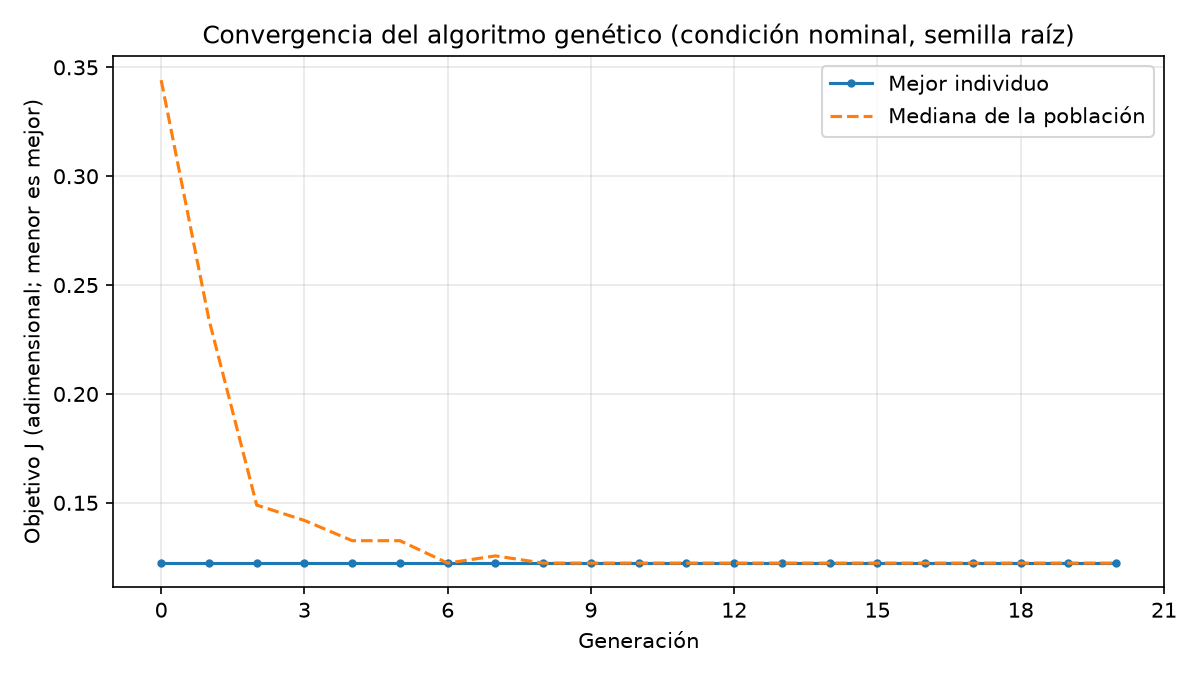
\includegraphics[width=0.75\textwidth]{figuras/convergencia_genetico.png}
\caption{Convergencia del algoritmo genético (condición nominal, semilla raíz). El mejor individuo ya es óptimo desde la población inicial; la mediana de la población converge a él en unas 8 generaciones. El algoritmo se detiene tras 20 generaciones sin mejora.}
\label{fig:convergencia}
\end{figure}

\subsection{Selección del modelo de demanda}

Para no usar 2023--2024, el modelo se eligió con un protocolo congelado antes de ejecutarlo (\cod{docs/protocolo\_demanda.md}). Se compararon tres candidatos con un backtest de origen móvil y horizonte de 2 años, igual al de la validación~\cite{hyndman}:
\begin{itemize}[nosep]
  \item \textbf{M0:} tasa estable de todo el periodo de entrenamiento.
  \item \textbf{M1:} tasa de los últimos 3 años.
  \item \textbf{M2:} modelo log-lineal Poisson con intercepto por municipio y tendencia común.
\end{itemize}
Un modelo más complejo solo se elegía si reducía el WAPE de M0 en al menos 10\,\%.

\begin{table}[htbp]
\centering
\small
\begin{tabular}{lrrr}
\toprule
Pliegue (entrenamiento $\to$ prueba) & M0 & M1 & M2 \\
\midrule
1 (2015--2018 $\to$ 2019--2020) & 0.374 & 0.369 & 0.352 \\
2 (2015--2019 $\to$ 2020--2021) & 0.294 & 0.337 & 0.374 \\
3 (2015--2020 $\to$ 2021--2022) & 0.221 & 0.253 & 0.375 \\
\midrule
\textbf{WAPE promedio} & \textbf{0.297} & 0.320 & 0.367 \\
\bottomrule
\end{tabular}
\caption{Backtest del modelo de demanda (WAPE). Para calificar se exigía un WAPE $\le 0.267$; ni M1 ni M2 lo alcanzan, así que se elige M0.}
\label{tab:backtest}
\end{table}

\textbf{Distribución.} Con M0 ajustado en 2015--2022 ($n=88$, $p=11$), el índice de dispersión de Pearson es $\varphi=7.40$. La binomial negativa estima $a=0.116$, y la razón de verosimilitudes frente a Poisson da $p\approx10^{-72}$ (con corrección de frontera). Se cumplen las dos condiciones fijadas ($\varphi>1.5$ y $p<0.05$), así que se usa la binomial negativa~\cite{cameron}.

% ---------------------------------------------------------------------
\section{Comparación con la vida real}
\label{sec:real}

\subsection{Referencia real}

La referencia son los casos registrados por el MSPAS en Chiquimula en 2023 y 2024~\cite{mspas}: 11 municipios $\times$ 2 años $=22$ observaciones y 2{,}068 casos (934 y 1{,}134). Se descargaron el 22 de octubre de 2026 y se reservaron desde el inicio: no se usaron para ajustar ni elegir el modelo, los parámetros ni el algoritmo.

\subsection{Correspondencia del modelo base con la realidad}

\begin{table}[htbp]
\centering
\small
\begin{tabular}{lr}
\toprule
Métrica & Valor \\
\midrule
Casos observados / esperados & 2{,}068 / 1{,}285.3 \\
MAE municipal & 36.4 casos por municipio y año \\
WAPE & 0.387 \\
Sesgo & $-782.7$ casos ($-37.9\,\%$) \\
2023: observado / esperado & 934 / 645.8 \\
2024: observado / esperado & 1{,}134 / 639.5 \\
Spearman del ranking municipal & 0.938 \\
Coincidencia de los 3 municipios con más casos & 3/3 \\
\bottomrule
\end{tabular}
\caption{Validación del modelo de demanda contra los registros reservados.}
\label{tab:validacion}
\end{table}

\begin{figure}[htbp]
\centering
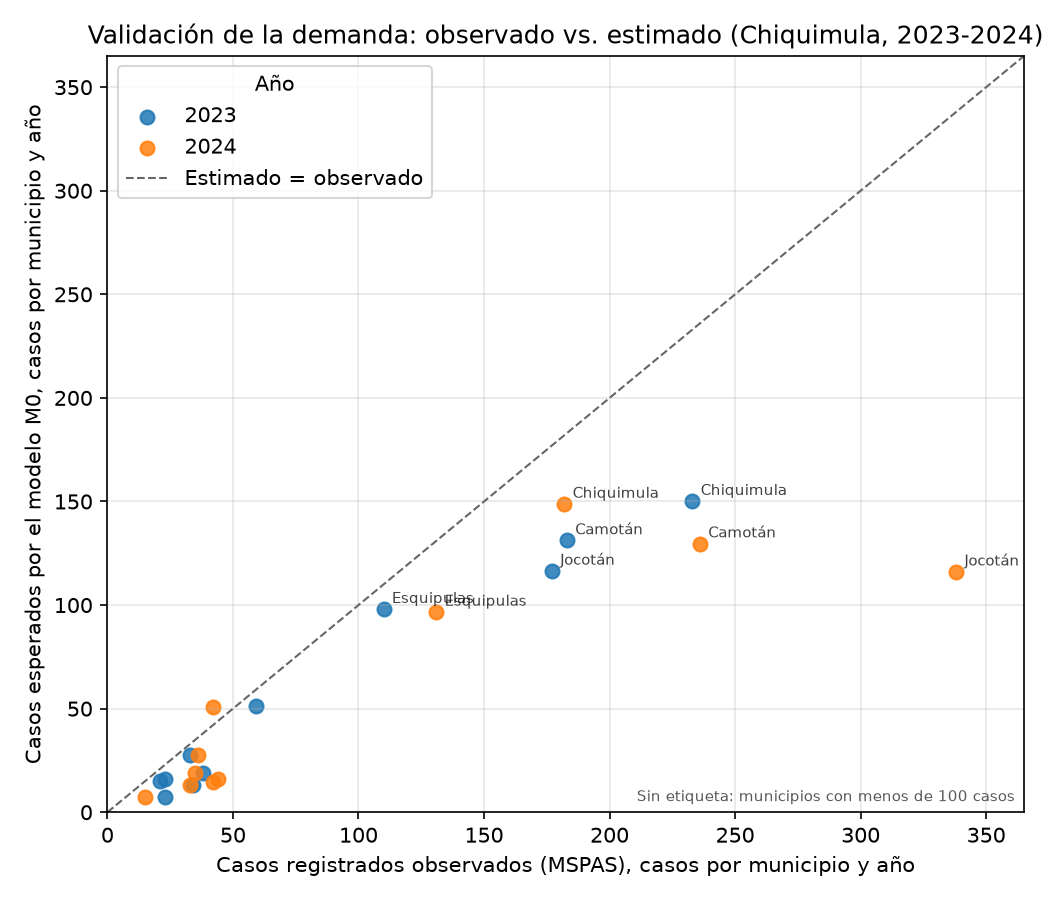
\includegraphics[width=0.72\textwidth]{figuras/validacion_demanda.png}
\caption{Casos observados frente a esperados por municipio y año, Chiquimula 2023--2024. La línea punteada indica estimado = observado; los puntos por debajo indican subestimación.}
\label{fig:validacion}
\end{figure}

\textbf{Interpretación.} El modelo \textbf{ordena bien} los municipios por carga (Spearman 0.938; acierta los tres de mayor demanda: Chiquimula, Jocotán y Camotán), pero \textbf{subestima el nivel} en un 37.9\,\%, más en 2024 que en 2023 (Figura~\ref{fig:validacion}). Es coherente con el aumento sistémico de 2023--2024 (Sección~\ref{sec:fuentes}), que ningún modelo podía anticipar con datos de 2015--2022. Para la simulación, la distribución relativa de la demanda entre municipios es confiable; el nivel absoluto no. Por eso la sensibilidad incluye una demanda $\times1.6$.

\subsection{Políticas evaluadas con la demanda real}

Ambas políticas, con las bases elegidas solo con datos de desarrollo y los parámetros nominales, se evaluaron con los casos reales de cada año (Tabla~\ref{tab:real}).

\begin{table}[htbp]
\centering
\small
\begin{tabular}{lrrrr}
\toprule
 & \multicolumn{2}{c}{2023 (934 casos)} & \multicolumn{2}{c}{2024 (1{,}134 casos)} \\
Política & Cobertura & Distancia media & Cobertura & Distancia media \\
\midrule
Base & 70.4\,\% & 2.1 km & 58.5\,\% & 0.9 km \\
Algoritmo genético & 71.0\,\% & 9.8 km & 58.5\,\% & 14.3 km \\
\midrule
Cambio & +0.5 pp (+0.8\,\%) & +7.8 km & 0.0 pp & +13.4 km \\
\bottomrule
\end{tabular}
\caption{Cobertura de los casos reales con una capacidad total de 663 casos/año.}
\label{tab:real}
\end{table}

\textbf{Interpretación.} Con la demanda real, la capacidad total (663) es muy inferior a los casos (934 y 1{,}134). En 2024 cualquier ubicación llena las tres brigadas (663/1{,}134 $=58.5\,\%$), y el algoritmo genético no puede mejorar la cobertura; incluso aumenta la distancia media, porque sus bases están en municipios de menor demanda propia. En 2023 la mejora es marginal (+0.5 pp). Por lo tanto, la ventaja que muestra la simulación (Sección~\ref{sec:resultados}) depende de que la capacidad sea comparable con la demanda: \textbf{con el nivel de demanda real de 2023--2024, el algoritmo genético no ofrece una mejora apreciable de cobertura.}

\subsection{Qué valida y qué no}

Esta comparación valida la aproximación de la \textbf{demanda municipal agregada de casos registrados} y evalúa ambas políticas con esa demanda. No valida tiempos de atención, capacidad real de las brigadas, resultados clínicos, prevalencia ni reducción de la desnutrición. Cualquier mejora reportada es una \textbf{mejora simulada de cobertura territorial}, no una mejora sanitaria observada.

% ---------------------------------------------------------------------
\section{Resultados}
\label{sec:resultados}

\subsection{Comportamiento del sistema}

\begin{figure}[htbp]
\centering
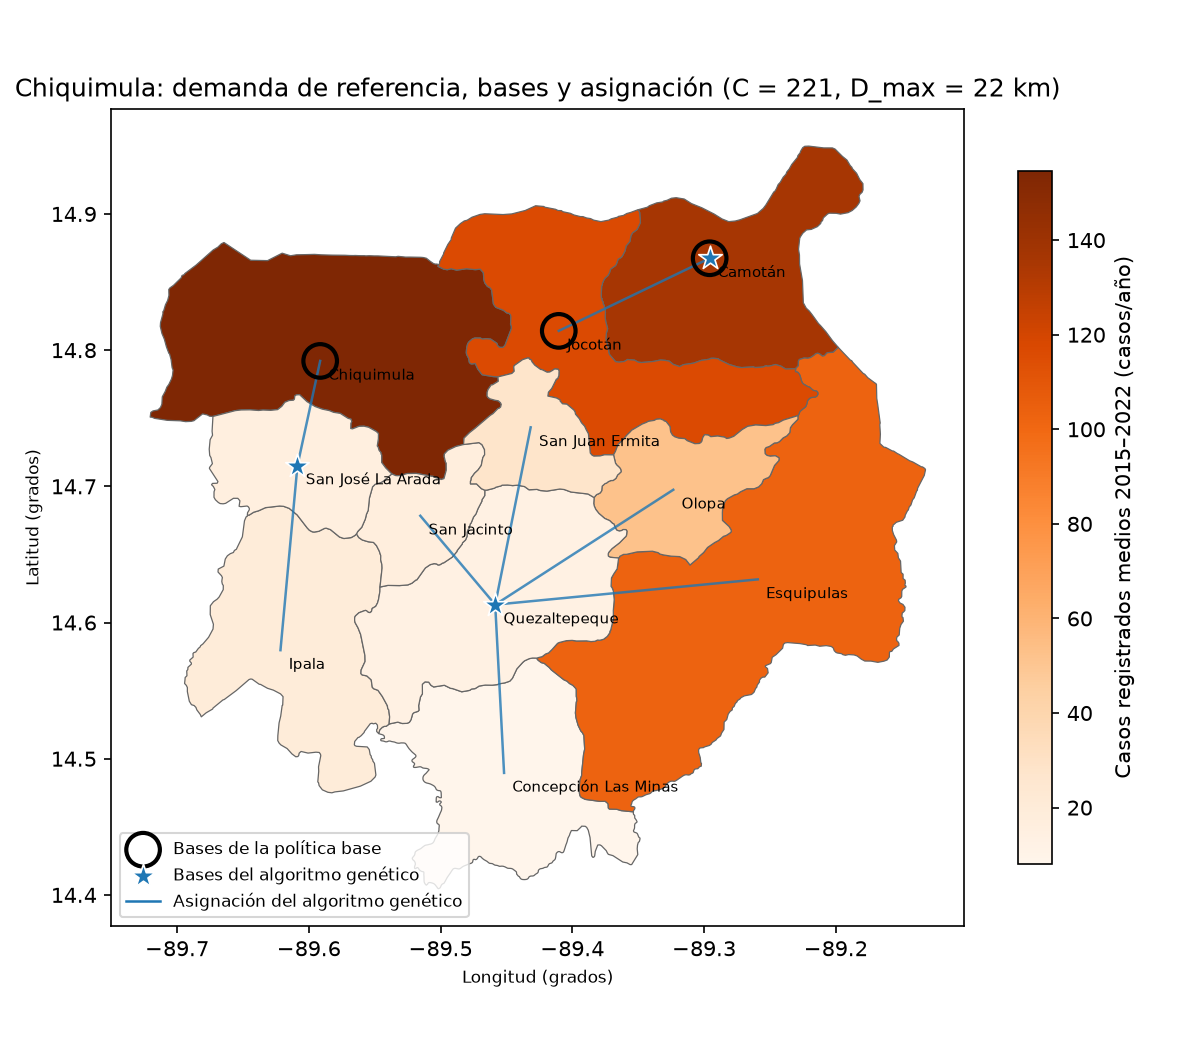
\includegraphics[width=0.78\textwidth]{figuras/mapa_asignacion.png}
\caption{Chiquimula con la demanda de referencia por municipio (casos medios 2015--2022), las bases de la política base (círculos), las del algoritmo genético en la condición nominal (estrellas) y las asignaciones del algoritmo (líneas).}
\label{fig:mapa}
\end{figure}

La política base ubica las brigadas en los tres municipios con más casos (Chiquimula, Jocotán y Camotán). Cada una se llena casi solo con su propio municipio (distancia media de 3.0 km) y deja sin cobertura a los municipios del sur. El algoritmo genético elige \textbf{San José La Arada, Camotán y Quezaltepeque} (Figura~\ref{fig:mapa}): municipios de menor demanda pero más céntricos, desde los cuales cada brigada alcanza a varios vecinos dentro de 22 km. En las otras condiciones el óptimo cambia: con capacidad 177 elige Chiquimula, Camotán y Esquipulas, y con radio de 40 km, Chiquimula, Jocotán y Olopa.

\subsection{Comparación de escenarios y sensibilidad}

\begin{table}[htbp]
\centering
\small
\begin{tabular}{lrrrrr}
\toprule
Condición & Base & Genético & Diferencia (pp) & IC 95\,\% (pp) & Cambio \\
\midrule
Nominal & 77.7 (4.2) & 92.0 (5.9) & +14.3 & [11.7, 16.8] & +18.4\,\% \\
Demanda $\times1.2$ & 75.9 (5.2) & 84.5 (8.3) & +8.6 & [6.1, 11.1] & +11.4\,\% \\
Demanda $\times1.6$ & 63.6 (7.2) & 65.3 (9.8) & +1.8 & [0.3, 3.3] & +2.8\,\% \\
Capacidad 177 & 74.3 (4.8) & 78.6 (7.8) & +4.2 & [1.8, 6.7] & +5.7\,\% \\
Radio 40 km & 96.9 (4.0) & 97.0 (4.0) & +0.2 & [$-0.01$, 0.32] & +0.2\,\% \\
\bottomrule
\end{tabular}
\caption{Cobertura simulada media (desviación estándar) en \%, con 30 réplicas pareadas por condición. La diferencia es genético $-$ base; el cambio es relativo a la media de la base.}
\label{tab:resultados}
\end{table}

\begin{figure}[htbp]
\centering
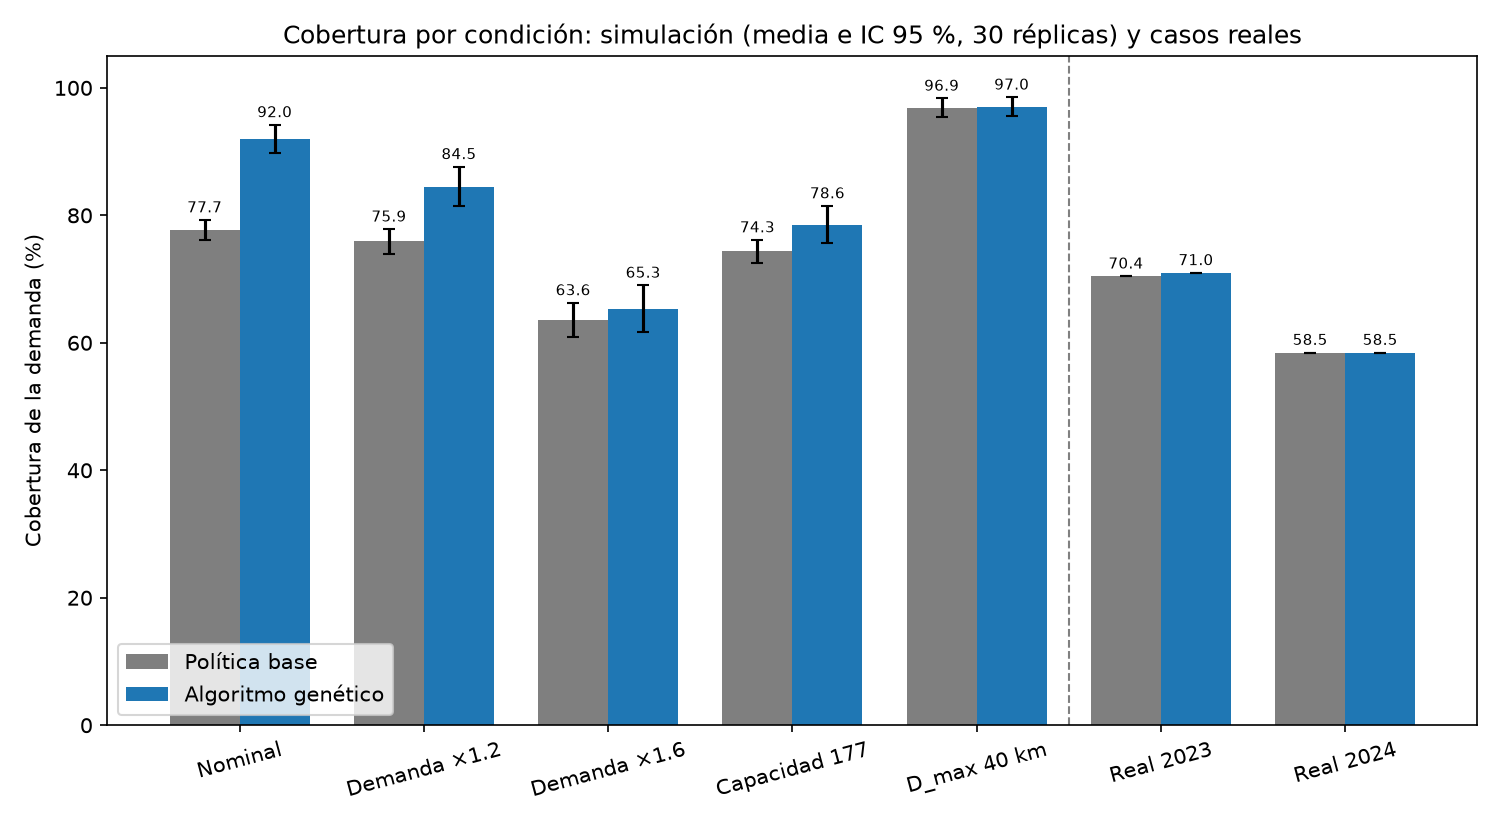
\includegraphics[width=\textwidth]{figuras/comparacion_escenarios.png}
\caption{Cobertura media por condición y política, con su intervalo de confianza del 95\,\% (30 réplicas), y cobertura de los casos reales de 2023 y 2024 (derecha de la línea punteada; sin intervalo, porque es una sola evaluación).}
\label{fig:comparacion}
\end{figure}

\begin{figure}[htbp]
\centering
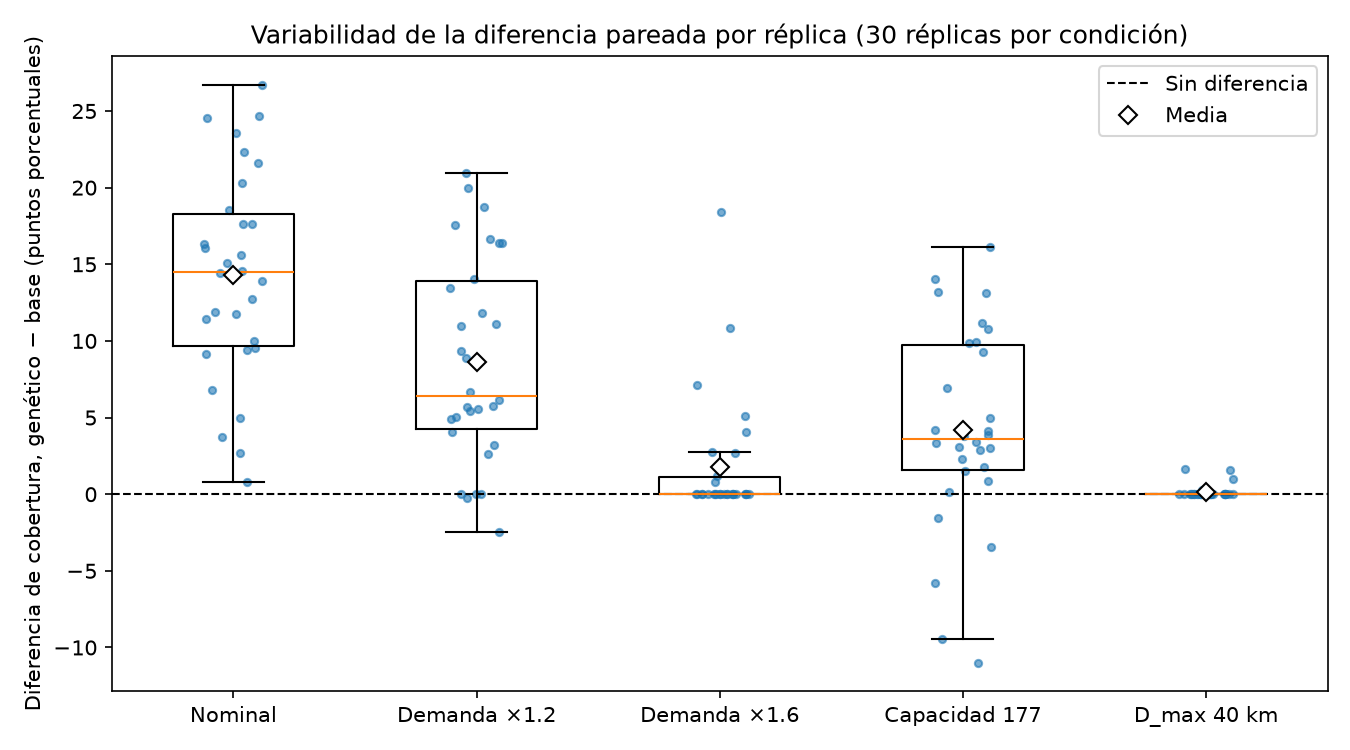
\includegraphics[width=0.85\textwidth]{figuras/diferencias_pareadas.png}
\caption{Diferencia de cobertura por réplica (genético $-$ base, en puntos porcentuales). Cada punto es una réplica; el diamante es la media.}
\label{fig:diferencias}
\end{figure}

\begin{itemize}
  \item \textbf{Nominal:} el algoritmo genético cubre 14.3 pp más que la base (IC 95\,\%: 11.7 a 16.8). En todas las réplicas la diferencia es positiva (Figura~\ref{fig:diferencias}).
  \item \textbf{Sensibilidad a la demanda:} la ventaja se reduce a 8.6 pp con $\times1.2$ y a 1.8 pp con $\times1.6$. Al crecer la demanda, la capacidad se satura y la ubicación importa menos.
  \item \textbf{Capacidad $-20\,\%$:} la ventaja baja a 4.2 pp, con más variabilidad. En 5 de las 30 réplicas la base cubre más (y en 2 con demanda $\times1.2$), porque el algoritmo decide con la demanda media y no con la de cada réplica.
  \item \textbf{Radio de 40 km:} casi todos los municipios quedan al alcance de cualquier base y las dos políticas cubren cerca del 97\,\%. La diferencia (+0.2 pp) no es estadísticamente distinta de cero.
  \item \textbf{Costo de la mejora:} la distancia media de atención sube de 3.0 a 11.0 km en la condición nominal, dentro del radio de 22 km. La peor cobertura municipal pasa de 0.00 a 0.45: el algoritmo deja menos municipios completamente desatendidos.
  \item \textbf{Tiempo de cómputo:} unos 42 ms por ejecución del algoritmo genético frente a 0.2 ms de la política base.
\end{itemize}

\subsection{Análisis adicional: escalabilidad del algoritmo genético}
\label{sec:escalabilidad}

En Chiquimula la enumeración basta, así que se diseñó y congeló un análisis adicional, antes de ejecutarlo (\cod{docs/analisis\_escalabilidad.md}), con instancias donde enumerar es costoso o imposible:

\begin{itemize}[nosep]
  \item \textbf{Huehuetenango}, $K=4$: 33 municipios, 40{,}920 combinaciones, óptimo exacto conocido.
  \item \textbf{País completo}, $K=10$, 20 y 40: 338 municipios y de $10^{18}$ a $10^{52}$ combinaciones.
\end{itemize}

Las reglas de capacidad son las del piloto; el radio es de 35 km en Huehuetenango (mediana de sus distancias) y de 22 km a escala nacional. Se compararon cuatro métodos sobre la demanda de referencia:
\begin{itemize}[nosep]
  \item la política base;
  \item una búsqueda voraz que agrega la base que más reduce $J$;
  \item una búsqueda aleatoria con \textbf{el mismo número de evaluaciones} que el algoritmo genético en cada semilla;
  \item el algoritmo genético con los \textbf{mismos parámetros congelados}.
\end{itemize}
Los métodos estocásticos se ejecutaron con 30 semillas.

\begin{table}[htbp]
\centering
\small
\begin{tabular}{lrrrrr}
\toprule
Instancia & Base & Voraz & Aleatoria & Genético & Gen.\ $-$ aleatoria (IC 95\,\%) \\
\midrule
Huehuetenango, $K=4$ & 83.6 & 98.0 & 99.0 & \textbf{99.6} & +0.6 pp [0.4, 0.9] \\
Nacional, $K=10$ & 35.4 & \textbf{50.0} & 39.0 & 47.9 & +8.9 pp [8.4, 9.4] \\
Nacional, $K=20$ & 46.9 & \textbf{67.4} & 51.8 & 63.7 & +11.9 pp [11.3, 12.4] \\
Nacional, $K=40$ & 64.1 & \textbf{81.0} & 64.1 & 76.7 & +12.5 pp [12.0, 13.1] \\
\bottomrule
\end{tabular}
\caption{Cobertura media de la demanda de referencia (\%) por método. En Huehuetenango el óptimo exacto tiene $J=0.0558$; el algoritmo genético lo alcanzó en 3 de 30 ejecuciones (J medio 0.076, frente a 0.166 del voraz).}
\label{tab:escalabilidad}
\end{table}

\begin{figure}[htbp]
\centering
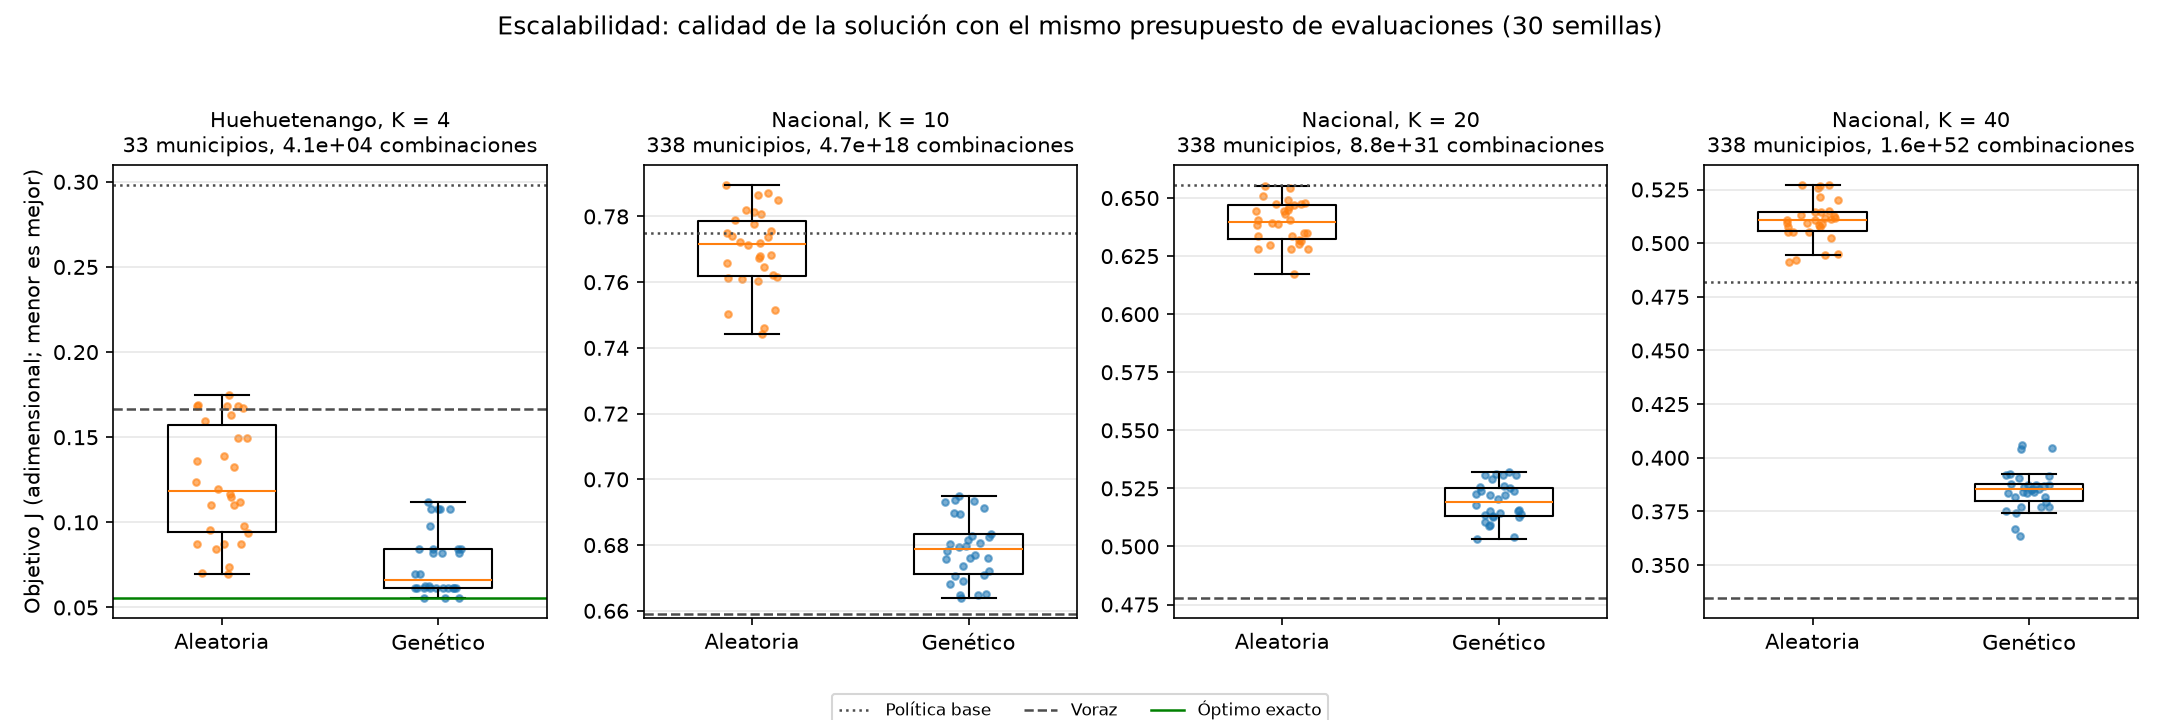
\includegraphics[width=\textwidth]{figuras/escalabilidad.png}
\caption{Objetivo $J$ (menor es mejor) por método e instancia. Las cajas muestran las 30 semillas de la búsqueda aleatoria y del algoritmo genético; las líneas, la política base, el voraz y, en Huehuetenango, el óptimo exacto.}
\label{fig:escalabilidad}
\end{figure}

\begin{itemize}
  \item \textbf{Frente a la búsqueda aleatoria con el mismo presupuesto,} el algoritmo genético gana en 118 de 120 pares, y la ventaja crece con el tamaño del problema. Con $K=40$, la búsqueda aleatoria es incluso peor que la política base. La búsqueda guiada del algoritmo sí aporta.
  \item \textbf{Frente a la política base,} cubre entre 12 y 17 pp más a escala nacional.
  \item \textbf{Frente al voraz:} en Huehuetenango gana el algoritmo genético, pero \textbf{a escala nacional gana el voraz} (brecha del genético del 3 al 15\,\% en $J$), que usa entre 1.8 y 4 veces más evaluaciones.
  \item \textbf{Con los parámetros congelados,} el algoritmo evalúa solo el 1.2\,\% del espacio de Huehuetenango y alcanza el óptimo en 3 de 30 ejecuciones. Más población y generaciones, o sembrar la población inicial con la solución voraz, son mejoras naturales que no se probaron.
\end{itemize}

% ---------------------------------------------------------------------
\section{Propuesta: cuántas brigadas para identificar cuántos casos}
\label{sec:propuesta}

Los experimentos anteriores fijan 3 brigadas y preguntan dónde ubicarlas. Para proponer un sistema hay que responder antes \emph{cuántas brigadas hacen falta}. Para eso la capacidad de una brigada tiene que expresarse en una unidad con respaldo.

\subsection{Qué hace una brigada: evidencia}

\begin{itemize}
  \item \textbf{Productividad:} según el PMA, cada brigada de salud y nutrición ``realiza una evaluación de 20 a 35 niñas y niños'' por día, en jornadas de 8:00 a 15:00 (San Marcos, 2020)~\cite{pma2020}.
  \item \textbf{Proporción de casos:} en Huehuetenango, 13 brigadas evaluaron a 13{,}433 menores de cinco años y detectaron 257 casos de desnutrición aguda moderada o severa, el 1.9\,\%~\cite{unicef2020}. En Alta Verapaz, 19 brigadas monitorearon a 5{,}574 niños y detectaron 21 casos, el 0.4\,\%~\cite{ops2022}.
\end{itemize}

Una brigada \textbf{evalúa niños} y, al evaluarlos, \textbf{identifica casos}. Expresar su capacidad en ``casos atendidos por año'', como en una primera versión de este estudio, no tiene respaldo. Esa versión (\cod{docs/estudio\_dimensionamiento.md}) se conserva en el repositorio como antecedente.

\subsection{Diseño}

El estudio se congeló antes de ejecutarlo (\cod{docs/estudio\_tamizaje.md}).
\begin{itemize}
  \item \textbf{Demanda de evaluación:} los niños de 0 a 4 años de 2024 por municipio (INE; 50{,}904 en total), con una ronda de tamizaje al año (supuesto).
  \item \textbf{Capacidad por brigada:} 20, 27.5 o 35 evaluaciones por día (PMA) $\times$ 220 días de campo (supuesto), es decir 4{,}400, 6{,}050 o 7{,}700 evaluaciones al año.
  \item \textbf{Casos identificados:} niños evaluados en cada municipio $\times$ tasa de casos de 2024 de ese municipio. La tasa aproxima dónde es más probable encontrar casos.
  \item \textbf{Decisión:} cuántas brigadas tienen base en cada municipio. \textbf{Varias pueden compartir municipio.}
  \item \textbf{Reparto óptimo:} para una ubicación dada, qué niños evalúa cada brigada (solo dentro del tiempo máximo de viaje por carretera de OSRM~\cite{osrm,osm}) se resuelve como un \textbf{programa lineal}, de forma óptima.
  \item \textbf{Dos objetivos:} \emph{identificar casos} (principal: maximizar los casos esperados) y \emph{evaluar niños} (alternativo: maximizar los niños evaluados, sin importar la tasa).
  \item \textbf{Factores:} de 1 a 15 brigadas, las tres productividades y un viaje máximo de 45, 60 o 90 minutos (270 configuraciones).
  \item \textbf{Búsqueda de la ubicación:}
    \begin{itemize}[nosep]
      \item enumeración exacta hasta 5 brigadas (hasta 3{,}003 ubicaciones);
      \item heurística voraz;
      \item el algoritmo genético del proyecto, generalizado para admitir varias brigadas por municipio (5 semillas por configuración).
    \end{itemize}
\end{itemize}

\subsection{Cuántas brigadas hacen falta}

\begin{table}[htbp]
\centering
\small
\begin{tabular}{lcccc}
\toprule
Productividad & Capacidad anual & 50\,\% de los casos & 80\,\% & 90\,\% \\
\midrule
20 evaluaciones/día & 4{,}400 & 5 (59\,\%) & 8 (81--82\,\%) & 10 (93\,\%) \\
\textbf{27.5 evaluaciones/día} & \textbf{6{,}050} & \textbf{3 (50\,\%)} & \textbf{6 (83\,\%)} & \textbf{7 (91\,\%)} \\
35 evaluaciones/día & 7{,}700 & 3 (61\,\%) & 5 (86\,\%) & 6 (96\,\%) \\
\bottomrule
\end{tabular}
\caption{Menor número de brigadas que identifica cada meta de los casos esperados de 2024 (objetivo principal). El resultado es el mismo con viajes de hasta 45, 60 o 90 minutos.}
\label{tab:tamizaje}
\end{table}

\begin{figure}[htbp]
\centering
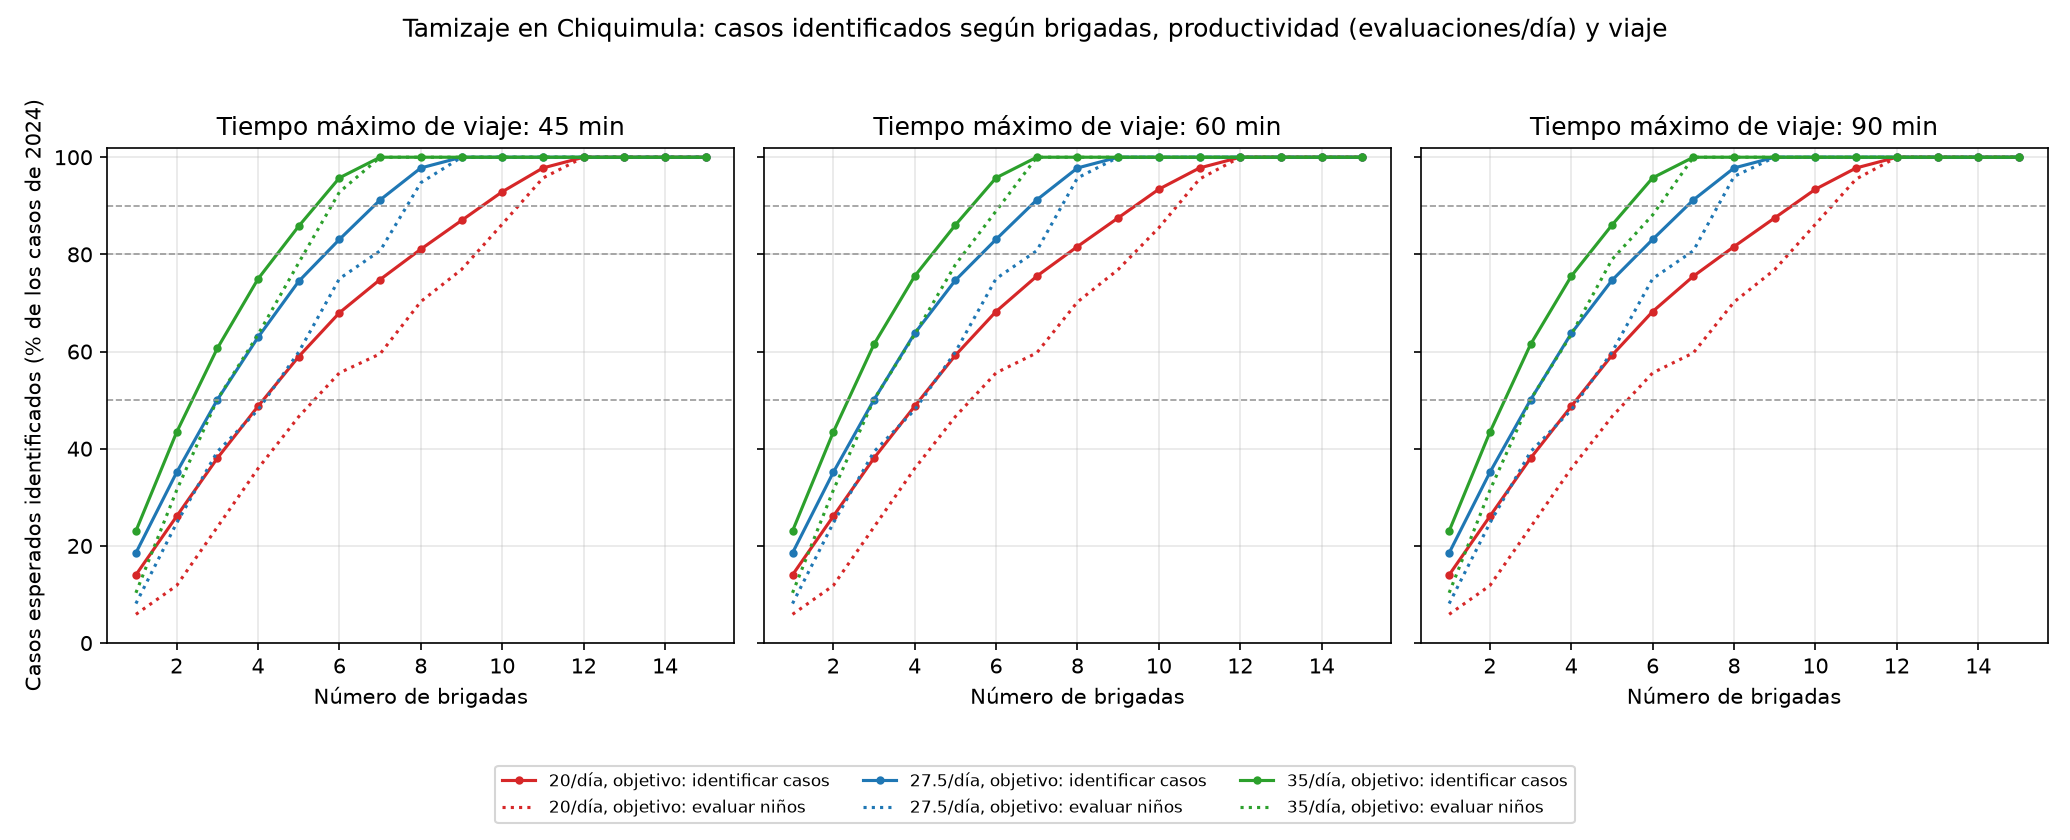
\includegraphics[width=\textwidth]{figuras/tamizaje_curvas.png}
\caption{Casos esperados identificados según el número de brigadas, para cada productividad y tiempo máximo de viaje. Líneas continuas: objetivo de identificar casos; punteadas: objetivo de evaluar niños. Líneas horizontales: metas de 50, 80 y 90\,\%.}
\label{fig:tamizaje}
\end{figure}

\begin{itemize}
  \item \textbf{El número de brigadas depende sobre todo de su productividad:} entre 5 y 8 brigadas para identificar el 80\,\% de los casos esperados.
  \item \textbf{El tiempo de viaje casi no cambia la respuesta:} la capacidad de evaluación, no el acceso, es lo que limita.
  \item \textbf{Evaluar a todos los niños} una vez al año con 27.5 evaluaciones por día requiere unas 9 brigadas. La recomendación de evaluar cada mes requeriría unas 101 brigadas: la distancia entre lo deseable y lo factible justifica priorizar.
\end{itemize}

\subsection{Configuración de referencia}

Con 27.5 evaluaciones por día, viajes de hasta 60 minutos y la meta del 80\,\%, hacen falta \textbf{6 brigadas} (Tabla~\ref{tab:referencia}, Figura~\ref{fig:tamizaje_mapa}).

\begin{table}[htbp]
\centering
\small
\begin{tabular}{p{2.4cm}p{4.2cm}rrrr}
\toprule
Objetivo & Ubicación & Casos & Niños & Casos (tasas 2023) & Viaje \\
\midrule
\textbf{Identificar casos} & Jocotán $\times$2, Camotán $\times$2, Esquipulas, Quezaltepeque & \textbf{83.1\,\%} & 71.3\,\% & 73.3\,\% & 14.2 min \\
Evaluar niños & Chiquimula $\times$2, Jocotán $\times$2, Camotán, Esquipulas & 75.0\,\% & 71.3\,\% & 72.0\,\% & 1.3 min \\
\bottomrule
\end{tabular}
\caption{Planes con 6 brigadas según el objetivo. ``Casos'': casos esperados identificados respecto de los de 2024; ``Niños'': niños de 0 a 4 años evaluados.}
\label{tab:referencia}
\end{table}

\begin{figure}[htbp]
\centering
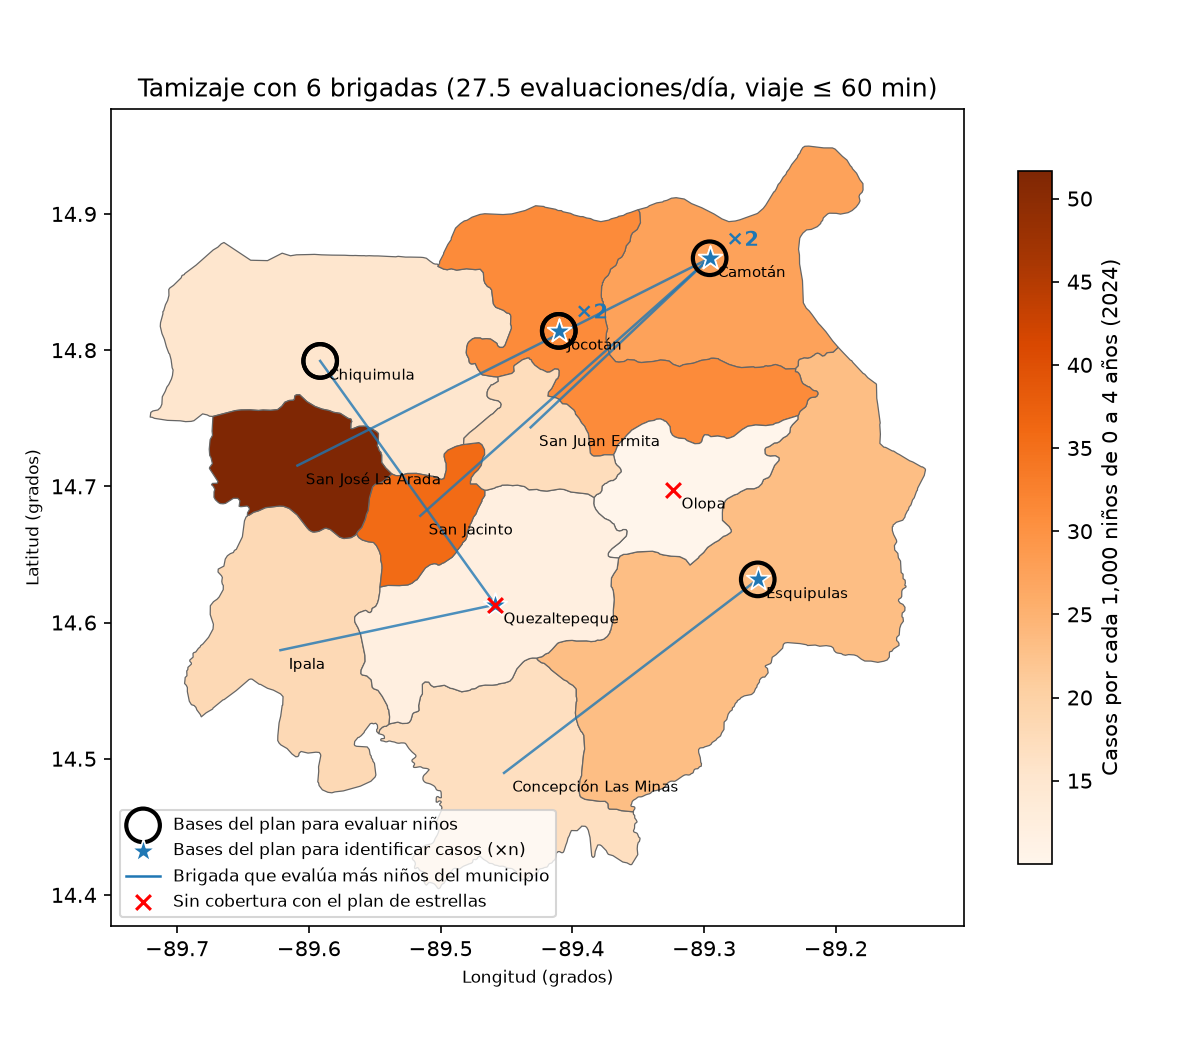
\includegraphics[width=0.72\textwidth]{figuras/tamizaje_mapa.png}
\caption{Configuración de referencia: 6 brigadas (27.5 evaluaciones por día, viaje de hasta 60 minutos). El color indica casos por cada 1{,}000 niños en 2024. Estrellas: bases del plan para identificar casos ($\times$n: brigadas en el municipio); círculos: bases del plan para evaluar niños (también con dos brigadas en Chiquimula y en Jocotán). La brigada con base en Quezaltepeque evalúa municipios vecinos con tasa más alta, no el suyo, que tiene de las tasas más bajas.}
\label{fig:tamizaje_mapa}
\end{figure}

\begin{itemize}
  \item \textbf{Mismos niños, más casos.} Los dos planes evalúan a la misma cantidad de niños (71.3\,\%, la capacidad completa), pero orientar las brigadas a los municipios con más tasa \textbf{identifica 8 puntos más de casos} (83.1 frente a 75.0\,\%).
  \item \textbf{El costo es el viaje.} El plan para identificar casos recorre 14.2 minutos de media frente a 1.3, y deja 3 municipios con menos de la mitad de sus niños evaluados, frente a 6 del otro plan.
  \item \textbf{Robustez:} con las tasas de 2023 el mismo plan identifica el 73.3\,\% de los casos de ese año. La ubicación depende en parte del año usado para planificar.
\end{itemize}

\subsection{Calidad de la búsqueda}

\begin{itemize}
  \item \textbf{Con 5 brigadas o menos,} el algoritmo genético alcanzó el óptimo exacto en 448 de 450 ejecuciones (99.6\,\%).
  \item \textbf{Con más brigadas,} donde la enumeración ya no es práctica (más de 180{,}000 ubicaciones con 10 brigadas), el mejor plan lo encontró el algoritmo genético en 103 de 180 configuraciones y la heurística voraz en 77. Por eso el plan propuesto toma el mejor de ambos.
  \item A diferencia del piloto de 3 brigadas, aquí el espacio de búsqueda sí justifica el algoritmo genético.
\end{itemize}

\subsection{Línea recta frente a carretera}

Por carretera, los trayectos entre municipios son en mediana \textbf{1.74 veces} más largos que en línea recta (39.6 frente a 22.3 km), con un tiempo mediano de 50 minutos. El orden de cercanía se conserva en buena medida (Spearman 0.83). Por tanto, los experimentos de las secciones anteriores, hechos en línea recta, subestiman las distancias reales, aunque la estructura de cercanía es parecida.

% ---------------------------------------------------------------------
\section{Limitaciones}
\label{sec:limitaciones}

\begin{itemize}
  \item \textbf{Casos registrados no son prevalencia:} dependen de la búsqueda activa y del registro. El aumento de 2023--2024 puede reflejar más casos, mejor registro o ambas cosas.
  \item \textbf{Ausencias:} el MSPAS no publica ceros explícitos; un municipio-año sin fila no se distingue de cero casos. En Chiquimula no hay ausencias.
  \item \textbf{Nivel de la demanda subestimado} en un 37.9\,\% en la validación. Con el nivel real, la ventaja simulada del algoritmo desaparece (Sección~\ref{sec:real}).
  \item \textbf{Población proyectada,} no censal: depende del censo 2018 conciliado por el INE.
  \item \textbf{Distancias geodésicas entre centroides} en los experimentos principales: por carretera, los trayectos son en mediana 1.74 veces más largos (Sección~\ref{sec:propuesta}). Esto afecta directamente a la mayor distancia que implica la solución del algoritmo. El estudio de dimensionamiento sí usa tiempos por carretera, pero de OSRM, que supone un automóvil en condiciones normales; en caminos rurales o con lluvia el viaje real puede ser mayor.
  \item \textbf{Supuestos de escenario} ($K$, $C$, $D_{\max}$, pesos) sin fuente oficial: los resultados dependen de ellos, como muestra la sensibilidad. En los experimentos principales, la capacidad $C$ es una unidad abstracta para comparar métodos. La interpretación operativa, en evaluaciones por día, está en la propuesta de tamizaje (Sección~\ref{sec:propuesta}).
  \item \textbf{Propuesta de tamizaje:}
    \begin{itemize}[nosep]
      \item la productividad proviene de un solo reporte del PMA (2020, niños de 0 a 10 años);
      \item los 220 días de campo y la ronda única anual son supuestos;
      \item la tasa de 2024 subestima la prevalencia donde hubo poca búsqueda activa;
      \item \textbf{no se modela el seguimiento} de los casos detectados, porque no se encontró información pública sobre cuántos puede acompañar una brigada.
    \end{itemize}
  \item \textbf{Regla de asignación heurística} en los experimentos principales: no divide la demanda de un municipio entre brigadas y no garantiza la asignación óptima para unas bases dadas. La propuesta de tamizaje la reemplaza por un reparto óptimo mediante programación lineal.
  \item \textbf{Algoritmo genético:} no garantiza el óptimo global y sus parámetros no se calibraron. En el piloto la enumeración bastaría, y a escala nacional una heurística voraz encuentra mejores soluciones (Sección~\ref{sec:escalabilidad}).
  \item \textbf{Conocimiento previo:} el equipo vio totales agregados de 2023--2024 durante el perfil de calidad, antes de modelar. Se mitigó fijando de antemano los protocolos de demanda, parámetros y diseño experimental.
  \item \textbf{Un solo departamento piloto:} los resultados no se generalizan al país.
\end{itemize}

% ---------------------------------------------------------------------
\section{Conclusiones}
\label{sec:conclusiones}

\begin{itemize}
  \item \textbf{Respuesta a la pregunta de investigación.} Bajo los datos, supuestos y restricciones declarados, elegir las bases con el algoritmo genético en lugar de con la heurística de mayor demanda aumenta la cobertura simulada en \textbf{14.3 pp} (IC 95\,\%: 11.7 a 16.8) en la condición nominal. La clave es ubicar las brigadas en municipios céntricos que alcancen a varios vecinos, no en los de mayor demanda propia.
  \item \textbf{La mejora es condicional.} Depende de que la capacidad sea comparable con la demanda y de que la distancia limite. Se reduce con demanda $\times1.6$ (+1.8 pp), desaparece con un radio amplio (+0.2 pp, no significativa) y, con el nivel real de casos de 2023--2024, es de +0.5 y 0.0 pp. Con la demanda real, el factor limitante es la capacidad total, no la ubicación.
  \item \textbf{La mejora tiene un costo:} mayor distancia media de atención (de 3.0 a 11.0 km en la condición nominal), a cambio de menos municipios completamente desatendidos.
  \item \textbf{El modelo de demanda} identifica correctamente dónde se concentra la carga (Spearman 0.938), pero no anticipa el aumento de 2023--2024 ($-37.9\,\%$ de sesgo). Las conclusiones sobre ubicación son más confiables que las cifras absolutas de cobertura.
  \item \textbf{El algoritmo genético} alcanzó el óptimo exacto en todas las ejecuciones del piloto, donde la enumeración también es viable. En problemas mayores supera ampliamente a la búsqueda aleatoria y a la política base, pero con sus parámetros actuales una heurística voraz lo supera a escala nacional. Ampliar sus parámetros o combinarlo con la solución voraz es el siguiente paso natural.
  \item \textbf{Propuesta para Chiquimula.} Con la productividad documentada por el PMA, identificar el 80\,\% de los casos esperados requiere entre 5 y 8 brigadas (35 a 20 evaluaciones por día). En el escenario central, \textbf{6 brigadas (dos en Jocotán, dos en Camotán, una en Esquipulas y una en Quezaltepeque) identifican el 83\,\% de los casos}. Evaluar a todos los niños una vez al año requeriría unas 9.
  \item \textbf{Cuántas antes que dónde, y a quién priorizar.} El número de brigadas depende sobre todo de su productividad; el tiempo de viaje casi no lo cambia. Con una flota dada, orientar las brigadas a los municipios con más tasa identifica más casos (83 frente a 75\,\% con 6 brigadas), a cambio de más viaje y de dejar menos evaluados a los municipios de tasa baja. Elegir entre detección dirigida y vigilancia amplia es una decisión de política que el modelo hace explícita pero no resuelve.
\end{itemize}
\pendiente{Revisión final de las conclusiones por todo el equipo.}

% ---------------------------------------------------------------------
\section*{Declaración de uso de inteligencia artificial}
\addcontentsline{toc}{section}{Declaración de uso de inteligencia artificial}

El Integrante 1 usó Claude Code (Anthropic, modelo Claude Opus 5.5)~\cite{claudecode} como asistente para implementar los módulos de datos, demanda, algoritmo genético, experimentos, métricas y figuras, sus pruebas automatizadas, la documentación técnica y el borrador de este informe. El departamento piloto y la partición temporal provienen del plan del equipo. El protocolo de selección del modelo de demanda, la regla de recalibración de parámetros y el diseño experimental los propuso el asistente, y el equipo los aprobó y congeló antes de ejecutarlos. Los resultados se verificaron con pruebas automatizadas y con reproducción en un clon limpio del repositorio.
\pendiente{Integrantes 2 y 3: declarar si usaron herramientas de IA, cuáles y para qué. Si la planeación inicial del equipo se hizo con asistencia de IA, declararlo también.}

% ---------------------------------------------------------------------
\begin{thebibliography}{99}

\bibitem{mspas} Ministerio de Salud Pública y Asistencia Social (MSPAS). \emph{Morbilidad por desnutrición aguda (por departamento y municipio), años 2012 al 2024}. Portal de Datos Abiertos del MSPAS. \url{https://datosabiertos.mspas.gob.gt/dataset/desnutricion}. Consultado el 22 de octubre de 2026.

\bibitem{ine} Instituto Nacional de Estadística (INE), con apoyo de CEPAL y UNFPA. \emph{Municipal Population Projections of Guatemala by Age and Sex 2015--2030}. Publicado por UNFPA en Humanitarian Data Exchange. \url{https://data.humdata.org/dataset/municipal-population-projections-of-guatemala-by-age-and-sex-2015-2030}. Consultado el 22 de octubre de 2026.

\bibitem{codab} OCHA. \emph{Guatemala --- Subnational Administrative Boundaries (COD-AB)}. Humanitarian Data Exchange. \url{https://data.humdata.org/dataset/cod-ab-gtm}. Consultado el 22 de octubre de 2026.

\bibitem{codps} OCHA. \emph{Guatemala --- Subnational Population Statistics (COD-PS)}. Humanitarian Data Exchange. \url{https://data.humdata.org/dataset/cod-ps-gtm}. Consultado el 22 de octubre de 2026.

\bibitem{ensmi} Ministerio de Salud Pública y Asistencia Social (MSPAS), Instituto Nacional de Estadística (INE), Secretaría de Planificación y Programación de la Presidencia (Segeplán) e ICF International (2017). \emph{Encuesta Nacional de Salud Materno Infantil 2014--2015: Informe Final}. Rockville, Maryland. \url{https://dhsprogram.com/pubs/pdf/FR318/FR318.pdf}.

\bibitem{unicef2024} UNICEF Guatemala (25 de mayo de 2024). Comunicado de prensa sobre la visita de su embajadora de buena voluntad a las brigadas de salud y nutrición en Escuintla. \url{https://www.unicef.org/guatemala/comunicados-prensa/gaby-moreno-embajadora-de-buena-voluntad-de-unicef-en-guatemala-visit\%C3\%B3-escuintla}. Consultado el 8 de noviembre de 2026.

\bibitem{pma2020} Programa Mundial de Alimentos (18 de diciembre de 2020). \emph{Juventudes rurales a la cabeza de las brigadas de salud y nutrición}. \url{https://es.wfp.org/historias/juventudes-rurales-la-cabeza-de-las-brigadas-de-salud-y-nutricion}. Consultado el 8 de noviembre de 2026.

\bibitem{unicef2020} UNICEF Guatemala (16 de diciembre de 2020). \emph{En Guatemala, a la búsqueda de casos de desnutrición infantil ocultos por la pandemia}. \url{https://www.unicef.org/guatemala/historias/en-guatemala-la-b\%C3\%BAsqueda-de-casos-de-desnutrici\%C3\%B3n-infantil-ocultos-por-la-pandemia}. Consultado el 8 de noviembre de 2026.

\bibitem{ops2022} Organización Panamericana de la Salud (24 de octubre de 2022). \emph{Brigadas integrales de salud y nutrición: servicios de salud que llegan a las comunidades más remotas de Alta Verapaz}. \url{https://www.paho.org/es/noticias/24-10-2022-brigadas-integrales-salud-nutricion-servicios-salud-que-llegan-comunidades-mas}. Consultado el 8 de noviembre de 2026.

\bibitem{osrm} Luxen, D. y Vetter, C. (2011). Real-time routing with OpenStreetMap data. En \emph{Proceedings of the 19th ACM SIGSPATIAL International Conference on Advances in Geographic Information Systems}, 513--516. Servidor usado: \url{https://router.project-osrm.org}, consultado el 8 de noviembre de 2026.

\bibitem{osm} OpenStreetMap contributors. \emph{OpenStreetMap}, datos bajo licencia ODbL. \url{https://www.openstreetmap.org}.

\bibitem{cameron} Cameron, A.~C. y Trivedi, P.~K. (2013). \emph{Regression Analysis of Count Data} (2.ª ed.). Cambridge University Press.

\bibitem{hyndman} Hyndman, R.~J. y Athanasopoulos, G. (2021). \emph{Forecasting: Principles and Practice} (3.ª ed.). OTexts. \url{https://otexts.com/fpp3/}.

\bibitem{holland} Holland, J.~H. (1975). \emph{Adaptation in Natural and Artificial Systems}. University of Michigan Press.

\bibitem{goldberg} Goldberg, D.~E. (1989). \emph{Genetic Algorithms in Search, Optimization, and Machine Learning}. Addison-Wesley.

\bibitem{eiben} Eiben, A.~E. y Smith, J.~E. (2015). \emph{Introduction to Evolutionary Computing} (2.ª ed.). Springer.

\bibitem{deb2000} Deb, K. (2000). An efficient constraint handling method for genetic algorithms. \emph{Computer Methods in Applied Mechanics and Engineering}, 186(2--4), 311--338.

\bibitem{church} Church, R. y ReVelle, C. (1974). The maximal covering location problem. \emph{Papers of the Regional Science Association}, 32(1), 101--118.

\bibitem{pandas} McKinney, W. (2010). Data structures for statistical computing in Python. En \emph{Proceedings of the 9th Python in Science Conference}, 56--61.

\bibitem{numpy} Harris, C.~R. et al. (2020). Array programming with NumPy. \emph{Nature}, 585, 357--362.

\bibitem{scipy} Virtanen, P. et al. (2020). SciPy 1.0: fundamental algorithms for scientific computing in Python. \emph{Nature Methods}, 17, 261--272.

\bibitem{matplotlib} Hunter, J.~D. (2007). Matplotlib: a 2D graphics environment. \emph{Computing in Science \& Engineering}, 9(3), 90--95.

\bibitem{claudecode} Anthropic (2026). \emph{Claude Code} [herramienta de software, modelo Claude Opus 5.5]. \url{https://www.anthropic.com}.

\end{thebibliography}

% ---------------------------------------------------------------------
\section*{Contribuciones}
\addcontentsline{toc}{section}{Contribuciones}

\begin{table}[htbp]
\centering
\small
\begin{tabularx}{\textwidth}{>{\raggedright\arraybackslash}p{2.6cm}L}
\toprule
Integrante & Responsabilidades y aportes \\
\midrule
Integrante 1 \pend{nombre} & Requisitos de la guía; adquisición y verificación de datos (MSPAS, INE, HDX) con checksums; correspondencias territoriales; reporte de calidad; selección del departamento piloto; protocolo y modelo de demanda; validación contra 2023--2024; recalibración de parámetros; reproducibilidad (datos versionados). Además, sustituyendo la parte asignada al Integrante 3: diseño experimental, algoritmo genético, experimentos, métricas, figuras y documentación de la técnica. Borrador del informe. \\
Integrante 2 (Denis Rodríguez) & Contratos compartidos; matriz de distancias; regla de asignación capacitada y verificador independiente; política base; enumerador exacto; flujo de réplicas con semillas pareadas; caso conocido; pruebas de propiedades internas; documentación del modelo. \\
Integrante 3 \pend{nombre} & Asignado: algoritmo genético, experimentos, métricas y visualizaciones. Su commit del 7 de noviembre contenía scripts con valores de relleno no conectados al modelo; se reemplazaron por la implementación descrita (ver \cod{docs/contribuciones.md}). \pend{aporte en informe o presentación, si lo hay} \\
\bottomrule
\end{tabularx}
\caption{Registro de contribuciones.}
\end{table}

\pendiente{El equipo revisa y confirma la redacción de cada fila.}

\end{document}
